%%%%%%%%%%%%%%%%%%%%%%%%%%%%%%%%%%%%%%%%%%%%%%%%%%%%%%%%%%%%%%%%%%%%
%Imperial College
\documentclass[a4paper,11pt,twoside]{article}
\usepackage[left=2.5cm,right=2cm,top=2cm,bottom=2cm]{geometry}

%%%%%%%%%%%%%%%%%%%%%%%%%%%%%%%%%%%%%%%%%%%%%%%%%%%%%%%%%%%%%%%%%%%%%
% Paragraph
\usepackage[parfill]{parskip}

% Images
\usepackage{graphicx} 
\usepackage{caption}
\usepackage{subcaption}

% URLs
\usepackage{hyperref}

% Maths
\usepackage{amsmath}
\usepackage{xfrac}

% Clever referencing
\usepackage{cleveref}

%%%%%%%%%%%%%%%%%%%%%%%%%%%%%%%%%%%%%%%%%%%%%%%%%%%%%%%%%%%%%%%%%%%%%
\begin{document} 
\title{MCMC in Action: Applying the Metropolis-Hastings Algorithm to a Two
Dimensional Gaussian}

\date{\today} 
\author{Dakshina Scott} 
\maketitle

%%%%%%%%%%%%%%%%%%%%%%%%%%%%%%%%%%%%%%%%%%%%%%%%%%%%%%%%%%%%%%%%%%%%%
\begin{abstract} 
The Metropolis-Hastings algorithm was used to generate samples from a probability
distribution. The samples were used, via maximum likelihood estimates to
find Monte Carlo estimates for the parameters of the distribution.
\end{abstract}

%%%%%%%%%%%%%%%%%%%%%%%%%%%%%%%%%%%%%%%%%%%%%%%%%%%%%%%%%%%%%%%%%%%%
\tableofcontents

%%%%%%%%%%%%%%%%%%%%%%%%%%%%%%%%%%%%%%%%%%%%%%%%%%%%%%%%%%%%%%%%%%%%%
\section{Background} 
Markov Chain Monte Carlo (MCMC) can be used to solve problems which would
otherwise not be solvable - such as intractable integrations or sampling from
complicated multivariate probability distributions.  

While the idea of Monte Carlo simulations has been
around for much longer, MCMC has flourished since the rise of computers allowed
much larger simulations. It was originally developed by Metropolis et al. at Los Alamos in
1953 to investigate the equation of state for substances consisting of
individual interacting molecules \cite{metropolis}.  

\subsection{Monte Carlo Methods \& Ordinary Monte Carlo}
Monte Carlo methods use random numbers to solve problems.  A Monte Carlo method
may be more narrowly defined as
"representing the solution of a problem as a parameter of a hypothetical
population, and using a random sequence of numbers to construct a sample of the
population, from which statistical estimates of the parameter can be found"
\cite{halton}.  

Ordinary Monte Carlo uses a sequence of random, independent identically distibuted
numbers are used in

A very simple example is a Monte Carlo estimate of $\pi$. Assume we have a
circle of radius one, contained exactly within a square ranging [-1, 1]. The
probability of random points from a uniform distribution within this range
landing in the circle is given by:
\begin{equation}
	P(inside) = \frac{\text{area of circle}}{\text{area of square}} =
	\frac{\pi}{4}.
\end{equation}
As there are only two possible outcomes for each simulation - a point lands
either inside or outside of the circle - a  population of N points can be
described by a binomial distribution in which a 'success' is a point landing within
the circle:
\begin{equation}
	I \sim \mathcal{B}(N, \theta)
\end{equation}
where $\theta = P(\text{inside})$, and $I$ is the number of successes.
Thus we have represented the solution of our problem as a parameter of a
hypothetical population, that is a binomial population with unknown probability
of success.
We can estimate $\theta$ using its maximum-likelihood estimate \cite{som}, based
on the number of success we observed in our random sampling:
\begin{equation}
	\theta = \frac{I}{N},
\end{equation}

So a Monte Carlo estimate for $\pi$ is given by
\begin{equation}
	\pi_{MC} = 4 \theta = 4 \frac{I}{N}.
\end{equation}

\subsection{Rejection Sampling}
Rejection sampling is a particular type of Monte Carlo method which can be used
if the target distribution can be evaluated, at least to within a normalization
constant. 

A random number $r$ is generated from some proposal distribution, $Q(\theta)$. A
corresponding random number is generated from a uniform distribution in the
range [0,$Q(\theta = r)$], representing a value on the y-axis. Both the
proposal distribution and the target distribution, $P(\theta|x)$ are
evaluated at this value. The probability of 'accepting' the sample is given by
$\frac{P(\theta = r|x)}{Q(\theta = r)}$ - in practice this is implemented by accepting the
sample if $y < P(\theta = r|x)$, and rejecting otherwise. The accepted points are
effectively a series of samples from the target distribution. From these
samples using the maximum-likelihood estimates for mean and variance gives the
Monte Carlo estimates for said quantities. It is important that $Q(\theta) >
P(\theta|x) \forall \, \theta$. 

\subsection{Markov Chains} 
\subsection{Metropolis-Hastings Algorithm}
\subsection{Examples of Applications}

\section{One-Dimensional Target Distribution} 
The posterior was found
for a quantity $\theta$, for the case of a Gaussian prior and a Gaussian
likelihood. With our knowledge of the distribution previously given by
$p(\theta)$, Bayes theorem gives us a way to update our knowledge given a new
set of measurements, $x$: 
\begin{equation}
	\label{eq:bayes}
	p(\theta|x) = \frac{p(x|\theta)p(\theta)}{p(x)},
\end{equation} 
where $p(\theta|x)$ is the posterior, our updated knowledge, $p(x|\theta)$ is
the likelihood of the data - the probability of observing those data as a
function of $\theta$, $p(\theta)$ is the prior distribution, i.e. our knowledge
before the measurements, and $p(x)$ is a normalizing constant.

Measurements were simulated by generating a set of independent, Gaussian
distributed variables, $\hat{\mathbf{x}} = \{x_1, x_2, ..., x_N\}$, representing observed
values for $\theta$. In this case we used that
\begin{equation}
	\label{eq:measurements}
	p(\theta) \sim \mathcal{N}(0.5, 0.1),
\end{equation}
in order to generate our results - i.e. that we have a population mean of 0.5,
and a population variance of 0.1. If the data $\hat{x}$ had come from an actual
experiment of course we would not know these two values. N values were
generated, resulting in a sample mean of $\bar{x} = 0.464$, and a sample
standard deviation of $\sigma = 0.075$.
The likelihood function for the data $\hat{x}$ is given by:

\begin{equation}
	\label{eq:rawlikelihood}
	\mathcal{L}(\theta) = p(\hat{\mathbf{x}}|\bar{x},\sigma) = \prod_{i=1}^{N} \frac{1}{\sqrt{2\pi}\sigma}\exp\left(-\frac{1}{2}\frac{(\theta - \hat{x}_i)^2}{\sigma^2}\right),
\end{equation}

from which it can be shown that:
\begin{equation}
	\label{eq:likelihood}
	\mathcal{L}(\theta) = L_0\exp\left(-\frac{1}{2}\frac{(\theta - \bar{x})^2}{\sfrac{\sigma^2}{N}}\right),
\end{equation}
where $L_0$ is a constant (see \cref{sec:likelihood}).

Assuming the following prior distribution:
\begin{equation}
	\label{eq:prior}
	p(\theta) =  \frac{1}{\sqrt{2\pi}}\exp\left(-\frac{1}{2}\frac{\theta^2}{\Sigma^2}\right),
\end{equation}
Bayes theorem can be used to find the posterior distribution.

\subsection{Analytical Solution}
In this case we have a simple gaussian prior and likelihood, and it can be shown
that the resulting posterior is also a gaussian (see \cref{sec:posterior}).
Because we know the form of the equation for a gaussian distribution, it can be
seen that the posterior mean and standard deviation are given by:
\begin{equation}
	\mu_{post} = \frac{\Sigma^2}{\sfrac{\sigma^2}{N} + \Sigma^2} \bar{x},
\end{equation}

\begin{equation}
	\sigma_{post} = \left( \frac{1}{\Sigma^2} + \frac{N}{\sigma^2} \right)^{-\frac{1}{2}}.
\end{equation}

This analytical solution gives us something to which our MCMC results can be
compared. However, in real world applications of MCMC, of course this would not
be available.

\subsection{Rejection Sampling} 
First a simple Monte Carlo method - rejection sampling - was applied to our toy
problem.
\begin{figure}[ht]
	\centering
	\begin{subfigure}[t]{0.4\textwidth}
		\centering
		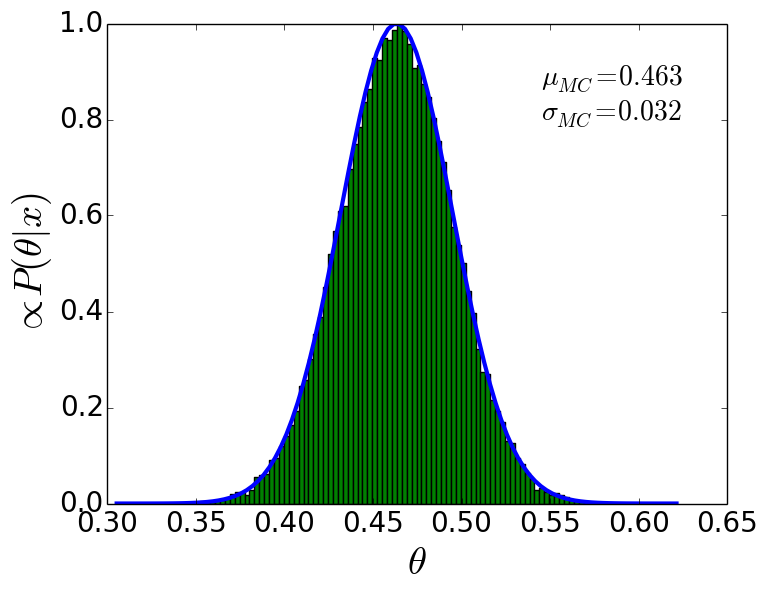
\includegraphics[width=\textwidth]{rejection.png}
		\caption{The histogram in green represents the distribution
			found by rejection sampling. The Monte Carlo mean and standard
			deviation are found to be $\mu_{MC} = 0.what$ and $\mu_{MC} = 0.0wat$.
			The blue line is the analytical distribution.}
		\label{fig:rejection}
	\end{subfigure}
	~
	\begin{subfigure}[t]{0.4\textwidth}
		\centering
		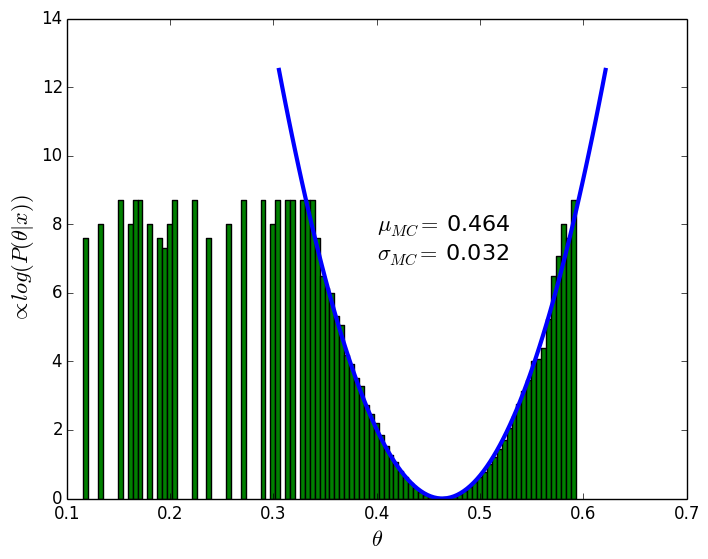
\includegraphics[width=\textwidth]{recentlog.png}
		\caption{A log-plot makes it easier to see the discrepencies at
			the extremeties of the plot. These are due to the finite
		domain over which samples are taken using this method.}
		\label{fig:rejlog}
	\end{subfigure}
\end{figure}

In \cref{fig:rejection}, the results appear to fit the analytical curve well.
However, plotting the logarithm of the results allows us to see clearly differences at
the edges of our Monte Carlo sample - this is because we can't take samples over
an infinite domain, and in this algorithm we must choose definite cut-off
points. The wider the domain the smaller the effect of this will be, but the
number of rejected candidate points will be larger. As there always has to be a
cut-off somewhere, this is an area where the Metropolis-Hastings algorithm will
be more effective (RANDOM WALK???). (AND ALSO ERROR - HOW DOES IT GO WITH MORE
DIMENSIONS??? - AND
EFFICIENCY???) (AND OTHER WAYS IT'S BETTER???).

\subsection{Metropolis-Hastings Algorithm} 
The Metropolis-Hastings algorithm was then applied to the same problem. 
\begin{figure}[ht]
	\centering
	\begin{subfigure}[t]{0.4\textwidth}
		\centering
		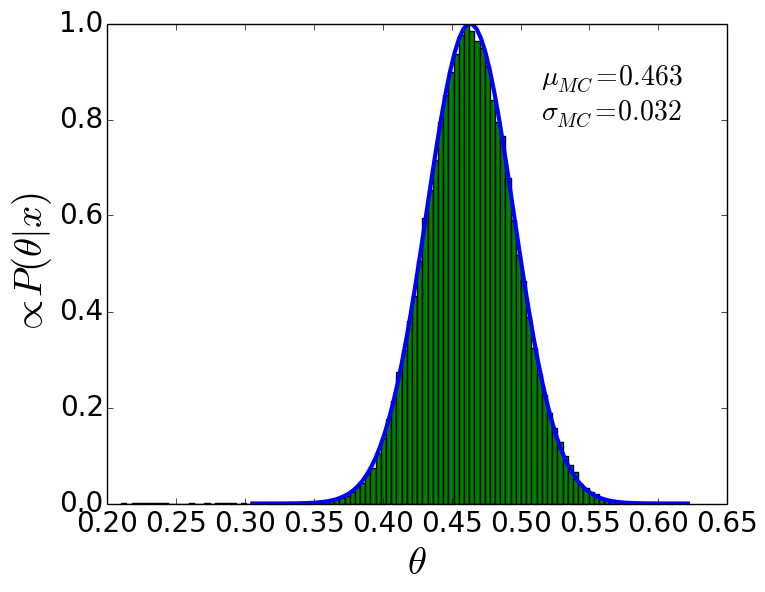
\includegraphics[width=\textwidth]{metropolishastings.png}
		\caption{The histogram in green represents the distribution
			found by the Metropolis-Hastings algorithm. The Monte Carlo mean and standard
			deviation are found to be $\mu_{MC} = 0.what$ and $\mu_{MC} = 0.0wat$.
			The blue line is the analytical distribution.}
		\label{fig:metropolis}
	\end{subfigure}
	~
	\begin{subfigure}[t]{0.4\textwidth}
		\centering
		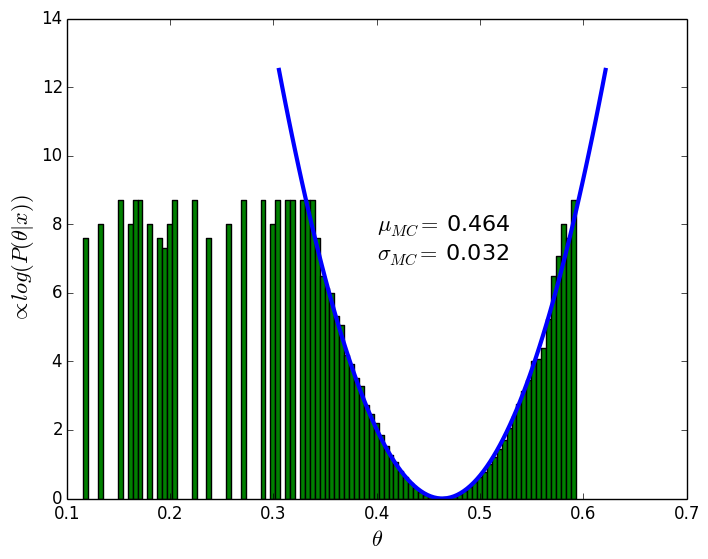
\includegraphics[width=\textwidth]{recentlog.png}
		\caption{A log-plot of the Metropolis-Hastings results shows
		that the sample is more consistent with the analytical solution,
	as compared with \cref{fig:rejlog}.}
		\label{fig:mhlog}
	\end{subfigure}
\end{figure}

BURN-IN??? - INC MULTIPLE STARTS CONVERGING

PROPOSAL SIGMA/ACCEPTANCE RATE???

MC SIGMA INDEPENDENT OF PROPOSAL SIGMA

\subsection{Analytical vs Rejection vs MH}

\section{Two-Dimensional Target Distribution} 
\subsection{Analytical Solution}
\subsection{Metropolis-Hastings} 
\subsection{Analytical vs MH}

\section{Conclusion}

%%%%%%%%%%%%%%%%%%%%%%%%%%%%%%%%%%%%%%%%%%%%%%%%%%%%%%%%%%%%%%%%%%%%%
\appendix 
\label{appendix}

\section{One-Dimensional Likelihood Function}
\label{sec:likelihood}
The likelihood distribution for a set of $N$ measurements is given by the product of the likelihood for each measurement:
\begin{align*}
	\mathcal{L}(\theta) &= \prod_{i=1}^{N} \frac{1}{\sqrt{2\pi}\sigma}\exp\left(-\frac{1}{2}\frac{(\theta - \hat{x}_i)^2}{\sigma^2}\right)
	\\ &= \left(\frac{1}{\sqrt{2\pi}\sigma}\right)^N \exp\left(-\frac{1}{2}\sum_{i=1}^{N}(\frac{\theta - \hat{x}_i)^2}{\sigma^2}\right).
\end{align*}
Taking, for now, just the exponent, and using that $\bar{x} = \frac{1}{N} \sum_i \bar{x}_i \Rightarrow \sum_i \hat{x}_i = N \bar{x}$:
\begin{align*}
	-\frac{1}{2\sigma^2}\sum_i^N(\theta - \hat{x})^2 &= -\frac{1}{2\sigma^2}(N\theta^2 - 2\theta \sum_i^N\hat{x}_i + \sum_i^N \hat{x}_i^2) 
	\\ &= -\frac{1}{2\sigma^2}(N\theta^2 - 2\theta N \bar{x} + \sum_i^N \hat{x}_i^2) 
	\\ &= -\frac{N}{2\sigma^2} (\theta^2 - 2\theta \bar{x} [ + \bar{x}^2 - \bar{x}^2]  + \frac{1}{N} \sum_i^N \hat{x}_i^2) 
	\\ &= -\frac{N}{2 \sigma^2} (\theta - \bar{x})^2 - \frac{N}{2 \sigma^2}(\frac{1}{N} \sum_{i=1}^{N} \hat{x}_i^2 - \bar{x}^2).
\end{align*}
So
\begin{align*}
	\mathcal{L}(\theta) &= \left( \frac{1}{\sqrt{2\pi}} \right)^N \exp \left(- \frac{N}{2 \sigma^2}(\frac{1}{N} \sum_{i=1}^{N} \hat{x}_i^2 - \bar{x}^2)\right) \exp \left(-\frac{N}{2 \sigma^2} (\theta - \bar{x})^2 \right)
	\\ &= L_0 \exp \left( -\frac{N}{2 \sigma^2} (\theta - \bar{x})^2 \right),
\end{align*}
where $L_0 = \left( \frac{1}{\sqrt{2\pi}} \right)^N \exp \left(- \frac{N}{2 \sigma^2}(\frac{1}{N} \sum_i \hat{x}_i^2 - \bar{x}^2)\right)$.

\section{Computing the Posterior Probability for Theta}
\label{sec:posterior}
Bayes theorem is given by:
\begin{align*}
	p(\theta|x) = \frac{p(x|\theta)p(\theta)}{p(x)}.
\end{align*}
Ignoring the normalization constant (as it is independent of $\theta$):
\begin{align*}
	p(\theta|x) \propto p(x|\theta)p(\theta).
\end{align*}
We have that
\begin{equation*}
	p(x|\theta) = L_0 \exp \left( -\frac{N}{2 \sigma^2} (\theta - \bar{x})^2 \right),
\end{equation*}
and
\begin{equation*}
	p(\theta) =  \frac{1}{\sqrt{2\pi}}\exp\left(-\frac{1}{2}\frac{\theta^2}{\Sigma^2}\right).
\end{equation*}

From these,
\begin{equation*}
	p(\theta|x) \propto \exp \left[ -\frac{1}{2} \left( \frac{(\theta - \bar{x})^2}{\sfrac{\sigma^2}{N}} +\frac{\theta^2}{\Sigma^2} \right) \right].
\end{equation*}

Taking just the exponent,
\begin{align*}
	\frac{(\theta - \bar{x})^2}{\sfrac{\sigma^2}{N}} + \frac{\theta^2}{\Sigma^2} &= \frac{N}{\Sigma^2\sigma^2} \left[\Sigma^2 (\theta - \bar{x})^2 + \frac{\sigma^2}{N} \theta^2 \right]
	\\ &= \left( \frac{1}{\Sigma^2} + \frac{N}{\sigma^2} \right) \left( \frac{1}{\sfrac{\sigma^2}{N} + \Sigma^2} \right) \left[ (\Sigma^2 + \frac{\sigma^2}{N})\theta^2 - 2\bar{x}\Sigma^2\theta + \Sigma^2\bar{x}^2 \right]
	\\ &= \left( \frac{1}{\Sigma^2} + \frac{N}{\sigma^2} \right) \left( \theta^2 - 2 \frac{\Sigma^2}{\sfrac{\sigma^2}{N} + \Sigma^2} \theta + \frac{\Sigma^2}{\sfrac{\sigma^2}{N} + \Sigma^2} \bar{x}^2 \right).
\end{align*}
The final term above is independent of $\theta$. Thus, as we are dealing with an exponent, we can subtract this term and add its square without losing proportionality. This allows us to complete the square so we have:
\begin{equation*}
	\left( \frac{1}{\Sigma^2} + \frac{N}{\sigma^2} \right) \left( \theta - \frac{\Sigma^2}{\sfrac{\sigma^2}{N} + \Sigma^2} \bar{x} \right)^2.
\end{equation*}

Putting this back inside the exponential we are left with:
\begin{equation*}
	p(\theta|x) \propto \exp \left[ -\frac{1}{2} \left( \frac{1}{\Sigma^2} + \frac{N}{\sigma^2} \right) \left( \theta - \frac{\Sigma^2}{\sfrac{\sigma^2}{N} + \Sigma^2} \bar{x} \right)^2 \right],
\end{equation*}

i.e. the posterior follows a Gaussian distribution with mean $\frac{\Sigma^2}{\sfrac{\sigma^2}{N} + \Sigma^2} \bar{x}$ and standard deviation $\left( \frac{1}{\Sigma^2} + \frac{N}{\sigma^2} \right)^{-\frac{1}{2}}$.

\section{Asymptotic Independence of Posterior on Prior}
For the posterior
\begin{equation*}
	p(\theta|x) \propto \exp \left[-\frac{1}{2} \frac{ \left( \theta - \frac{\Sigma^2}{\sfrac{\sigma^2}{N} + \Sigma^2} \bar{x} \right)^2}{ \left( \frac{1}{\Sigma^2} + \frac{N}{\sigma^2} \right)^{-1}} \right],
\end{equation*}
$
\begin{array}{l l l l}
	\text{as }N \rightarrow \infty, &\quad 
	\\ &\quad \left( \frac{1}{\Sigma^2} + \frac{N}{\sigma^2} \right)^{-1} &\rightarrow \frac{\sigma^2}{N} \quad &\left(\frac{N}{\sigma^2} \gg \frac{1}{\Sigma^2}\right), 
	\\ &\quad \frac{\Sigma^2}{\sfrac{\sigma^2}{N} + \Sigma^2} \bar{x} &\rightarrow \bar{x} \quad &\left(\frac{\sigma^2}{N} \rightarrow 0\right),
\end{array}
$
and the posterior becomes
\begin{equation*}
	p(\theta|x) \propto \exp \left[-\frac{1}{2} \frac{(\theta - \bar{x})^2}{\sfrac{\sigma^2}{N}} \right], 
\end{equation*}
i.e. the likelihood.

\section{Asymptotic Convergence of the Posterior Mean to the MLE Mean for Theta}
The posterior mean is given by:
\begin{equation*}
	\langle \theta \rangle = \int_{-\infty}^{+\infty} \theta p(\theta|x) \mathrm{d} \, \theta.
\end{equation*}
Inserting our equation for the posterior for $N \rightarrow \infty$, we have
\begin{equation*}
	\langle \theta \rangle = \int_{-\infty}^{+\infty} \theta \exp \left[- \frac{1}{2} \frac{(\theta - \bar{x})^2}{\sfrac{\sigma^2}{N}} \right] \mathrm{d} \, \theta. 
\end{equation*}
Making the substitution $y = \theta - \bar{x}$:
\begin{align*}
	\langle \theta \rangle &= \int_{-\infty}^{+\infty} (y+\bar{x})  \exp \left[- \frac{1}{2} \frac{y^2}{\sfrac{\sigma^2}{N}} \right] \mathrm{d} \, y
	\\ &= \int_{-\infty}^{+\infty} \bar{x} \exp \left(- \frac{1}{2}\frac{N}{\sigma^2} y^2 \right) \mathrm{d} \, y,
\end{align*}
as $ y \exp \left(- \frac{1}{2}\frac{N}{\sigma^2} y^2 \right) $ is an odd function.

Substituting back:
\begin{align*}
	\int_{-\infty}^{+\infty} \bar{x} \exp \left[- \frac{N}{\sigma^2} (\theta - \bar{x})^2 \right] \mathrm{d} \, \theta &= \bar{x} \int_{-\infty}^{+\infty} p(\theta|x) \mathrm{d} \, \theta
	\\ &= \bar{x},
\end{align*}
as the integral of a pdf between infinite limits is equal to one. 
\section{onedcode} 
\label{sec:onedcode}

\section{twodcode}
\label{sec:twodcode}

%%%%%%%%%%%%%%%%%%%%%%%%%%%%%%%%%%%%%%%%%%%%%%%%%%%%%%%%%%%%%%%%%%%%
\begin{thebibliography}{10}


	\bibitem{metropolis}
		Metropolis et al. (1953) Equation of State Calculations by Fast
		Computing Machines. The Journal of Chemical Physics.
		[Online] 21 (6), 1087-1092. Available from: doi:
		10.1063/1.1699114 [Accessed 21 October 2013].

	\bibitem{applications}
		Diaconis, P., 2009. The Markov Chain Monte Carlo Revolution.
		Bull. Amer. Math. Soc., Vol. 46, pp. 179-205

	\bibitem{handbookch1}
		Geyer, C., J., 2011. Handbook of Markov Chain Monte Carlo.
		Chapman \& Hall/CRC, p.3
		
	\bibitem{halton}
		Halton, J., H., 1970. A Retrospective and Prospective Survey of
		the Monte Method. SIAM Rev., Vol. 12, No. 1, pp. 1-63
	
	\bibitem{som}
		Trotta, R., 2012. Statistics of Measurement: Summary Handout.
		Imperial College London, p. 14

\end{thebibliography}

\end{document}
